% 1977 年黑龙江初试卷第 8 题：直角三角形 ABC，∠C=90°，CD⊥AB，D 为垂足，∠1=∠BCD，∠2=∠ACD（按源卷第 2 页布局）
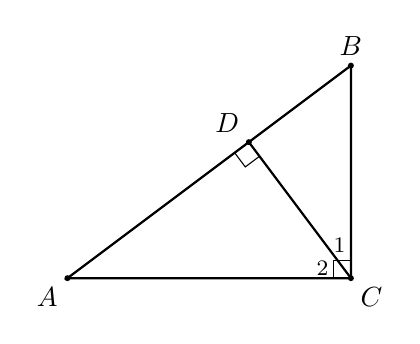
\begin{tikzpicture}[scale=0.9]
  \coordinate (A) at (0,0);
  \coordinate (C) at (4,0);
  \coordinate (B) at (4,3);
  \coordinate (D) at (2.56,1.92);
  \draw[thick] (A)--(B)--(C)--cycle;
  \draw[thick] (C)--(D);
  \draw (3.75,0)--(3.75,0.25)--(4,0.25);
  \draw (2.36,1.77)--(2.51,1.57)--(2.71,1.72);
  \fill (A) circle (1.2pt) node[below left] {$A$};
  \fill (B) circle (1.2pt) node[above] {$B$};
  \fill (C) circle (1.2pt) node[below right] {$C$};
  \fill (D) circle (1.2pt) node[above left] {$D$};
  \node at (3.84,0.47) {\footnotesize $1$};
  \node at (3.6,0.14) {\footnotesize $2$};
\end{tikzpicture}
